% !TEX encoding = UTF-8
% !TEX TS-program = pdflatex
% !TEX root = ../tesi.tex

%**************************************************************
\chapter{Tecnologie utilizzate}
\label{cap:Tecnologie utilizzate}
In questo capitolo seguirà un elenco delle tecnologie di riferimento adottate per la realizzazione dell'applicazione CS-Template.
\section{Frontend}
\subsection{Angular 6}
Angular è una piattaforam opensourse realizzato da Google nel 2016 che permette di creare le SPA, sfruttando i
pattern architetturali MVC e MVVM.
\\

Le applicazioni sviluppate in Angular vengono eseguite interamente dal web browser dopo essere state scaricate dal web server. Questo comporta il risparmio di dover spedire indietro la pagina web al web-server ogni volta che c'è una richiesta di azione da parte dell'utente. Il codice generato da Angular gira su tutti i principali web browser moderni.
\\

Ogni pagina web viene costruitta da diversi componenti. Un componente in Angular in generale è una piccola parte della view che reppressenta una specifica funzionalità(esempio la navbar).   Ogni component ha una propria logica
strutturale (scritta tramite appositi marcatori HTML), di presentazione (scritta con
appositi fogli di stile CSS oppure SCSS) e di business (scritta con il linguaggio di programmazione
TypeScript). Tutti i componenti possono comunicare tra di loro scambiandosi
oggetti, lo scambio viene fatto utilizzando diversi strumenti messi a disposizione da Angular. Oggi tale framework è alla versione 6.
\begin{figure}[!h] 
	\centering 
	
\includegraphics[width=0.4\columnwidth]{angular-logo} 
	\caption{Logo di Angular}
\end{figure}

\subsection{Angular material}
Angular material è una libreria che contiene una raccolta di componenti di Materia DesignG. Questo libreria è stata sviluppata sempre da Google e permette di realizzare delle UI molto avvanzata in maniena molto semplice. Fornendo una serie di semplici componenti(come i pulsanti, inputbox ecc) di Angular già fatta permette algli sviluppatori di risparmiare una notevole quantità di tempo. Tutti i componenti sono testati da Google garantendo cosi un corretto funzionamento.

\begin{figure}[!h] 
	\centering 
	
\includegraphics[width=0.4\columnwidth]{material}
	\caption{Logo di Material UI} 
\end{figure}


\subsection{Typescript} TypeScript è un linguaggio di programmazione libero ed Open source sviluppato da Microsoft basato su EMCAScript 6. Esso estende la sintassi di Javscript aggiungendo il concetto di tipizzazione(interfacce, classi, enum ecc). Questo lo rende molto simile ai linguaggi di programmmazione come Java oppure C++, e diventa anche molto semplice l'applicazione di molti design pattern conosciuti.
\\

 TypeScript nasce dal crescente bisogno di un linguaggio front-end per lo sviluppo di applicazioni JavaScript larga scala. Il linguaggio è nato dalla necessità di sicurezza e robustezza, sia da sviluppatori interni a Microsoft sia clienti. 
\begin{figure}[!h] 
	\centering 
	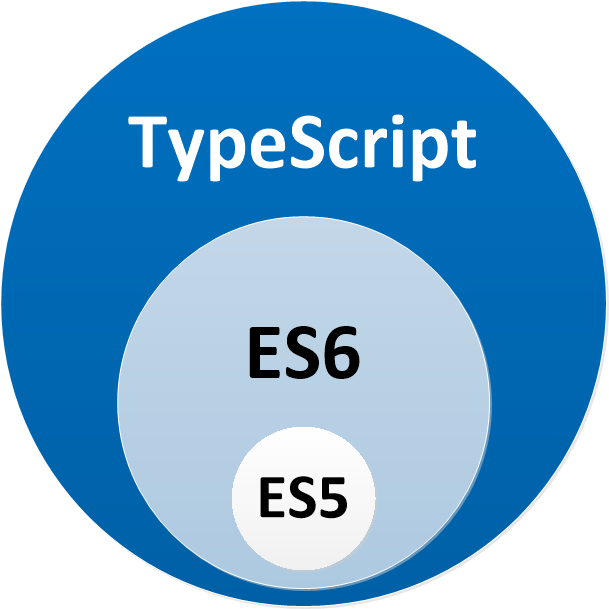
\includegraphics[width=0.4\columnwidth]{typescript} 
	\caption{Typescript rispetto ES6 e ES5}
\end{figure}


\subsection{HTML 5} L'HTML5 è un linguaggio di markup per la strutturazione delle pagine web, pubblicato come W3C Recommendation da ottobre 2014. HTML è stato usato come linguaggio per la definizione della logica strutturale del
front-end dell’applicazione. Una delle principali vantaggi di Angular sta proprio nel utilizzo di HTML pure rispetto i framework/librerie revali come React oppure Vue. 
\begin{figure}[!h] 
	\centering 
	
\includegraphics[width=0.4\columnwidth]{html} 
	\caption{Logo di HTML 5}
\end{figure}

\subsection{SASS} Sass (Syntactically Awesome StyleSheets) è un'estensione del linguaggio CSS che permette di utilizzare variabili, di creare funzioni e di organizzare il foglio di stile in più file.
\\

Il linguaggio Sass si basa sul concetto di preprocessore CSS, il quale serve a definire fogli di stile con una forma più semplice, completa e potente rispetto ai CSS e a generare file CSS ottimizzati, aggregando le strutture definite anche in modo complesso. SASS/CSS è un linguaggio utilizzato per definire la presentazione dell'applicazione. Poichè Angular Material fornisce molti componenti prefatti, questo linguaggio è utilizzato principalmente per definire il layout delle pagine. 
\begin{figure}[!h] 
	\centering 
	
\includegraphics[width=0.4\columnwidth]{sass}
	\caption{Logo di SASS}
\end{figure}

\section{Tecnologie Backend}
Per quanto riguarda il lato Backend è stato deciso di utilizzare il cloud computing. Esso è la distribuzione di servizi di calcolo, come server, risorse di archiviazione, database, rete, software, analisi e molto altro, tramite Internet ("il cloud"). 
\\

Le società che offrono questi servizi di calcolo sono dette provider di servizi cloud e in genere addebitano un costo per i servizi di cloud computing in base all'utilizzo(on demand). I provider più famosi oggigiorno sono Amazon, Microsoft e Google. 
\\

Dopo una breve analisi e confronto tra i servizi offerti da questi provider è stato deciso di utilizzare i servizi offerti da Amazon, ovvero gli AWS. La scelta è stata fatta soprattutto per la pololarità dei servizi Amazon, essendo Amazon primo a fornire questo tipo di servizio sono attualmente molto più utilizzati rispetto gli altri due. Per quanto riguarda i prezzi, quantità e qualità di servizi offerti da tuti i provider non è stato trovato un rirevante differenza. 
\begin{figure}[!h] 
	\centering 
	
\includegraphics[width=0.6\columnwidth]{ccaws}
	\caption{AWS cloud computing}
\end{figure} 
\subsection{Amazon Web Services}
Per l'applicazione in questione sono stati identificati specifici servizi di Amazon, che hanno permesso poi di realizzare un'archittettura serverless facilmente scalabile. In seguito è fornita una descrizione generale dei servizi scelti.

\subsection{AWS API Gateway} Amazon API Gateway è un servizio il cui scopo è quello di semplificare agli sviluppatori
la creazione, la pubblicazione, la manutenzione, il monitoraggio e la protezione
delle API su qualsiasi scala.
Questo servizio permette di creare un punto d'ingresso attraverso il quale le applicazioni posso accedere ai dati. Fornisce una API per ricevere le richiesta dalle applicazioni, dopo ogni richiesta questo servizio genera un evento che esegue qualcosa(una funzione lambda, un altra chiamata ecc).
\begin{figure}[!h] 
	\centering 
	
\includegraphics[width=0.2\columnwidth]{gateway}
	\caption{Logo API Gateway}
\end{figure}

\subsection{AWS Lambda} 

Sono delle semplici funzioni che ricevano come input un evento e possono ritornare qualche valore. Possono essere scritte in molti linguaggii dprogrammazione, come Nodejs(javascript), Java, C++ e Phython. 
\\

Queste funzioni possono comunicare con qualsiasi servizio di Amazon utilizzando AWS-SDK. In questo progetto sono state utilizzate diverse funzioni di questo tipo, princiaplamente per scrivere o leggere i dati su database.
\begin{figure}[!h] 
	\centering 
	
\includegraphics[width=0.5\columnwidth]{lambda}
	\caption{Logo di AWS Lambda}
\end{figure}  

\subsection{AWS DynomoDB} 
Amazon DynamoDB è un database non relazionale che fornisce prestazioni affidabili su qualsiasi scala. Si tratta di un database multi-master, multiregione e completamente gestito che fornisce latenza costante di pochi millisecondi e sicurezza integrata, backup e ripristino e cache in memoria.
\\

 Tutti i dati degli utenti e i tempalte sono stati salvati su questo database. L'acceso a tali avviene solo tramite le funzioni lambda.   
\begin{figure}[!h] 
	\centering 
	
\includegraphics[width=0.3\columnwidth]{dynamo}
	\caption{Logo di AWS DynamoDB}
\end{figure}

\subsection{AWS S3} 
Amazon Simple Storage Service è uno storage di
oggetti creato per memorizzare e ripristinare qualsiasi volume di dati da qualunque
origine: siti web, applicazioni per mobile o dati provenienti da diversi dispositivi. Può
essere utilizzato per memorizzare file multimediali ed è ideale per acquisire dati quali
foto, video o immagini di risoluzione elevata da dispositivi mobili, backup di dispositivi
mobile o computer.
\\

Nel contesto dello stage è stato utilizzato per garantire la persistenza di tutti i dati
non strutturati dell’applicazione. Inoltre l'applicazione stassa è stata caricata su questo servizio.   
\begin{figure}[!h] 
	\centering 
	
\includegraphics[width=0.4\columnwidth]{s3}
	\caption{Logo di AWS S3}
\end{figure}

\subsection{AWS Cognito} 
Amazon Cognito permette di aggiungere strumenti di registrazione, accesso e controllo degli accessi alle app Web e per dispositivi mobili in modo rapido e semplice. Amazon Cognito permette di ricalibrare le risorse per milioni di utenti e supporta l'accesso con provider di identità social quali Facebook, Google e Amazon 
\\

Nel contesto dello stage è stato utilizzato per garatire l'accesso alla pagina di amministratore solo agli utenti con le credenziali valide.   
\begin{figure}[!h] 
	\centering 
	
\includegraphics[width=0.4\columnwidth]{cognito}
	\caption{Logo di AWS Cognito}
\end{figure}

\section{Framework e le API di Zendesk}

\subsection{Zendesk Apps framework(ZAF)}
ZAF è un semplice framework sviluppato da Zendesk Inc. Viene utilizzato per realizzare le applicazione per la piattaforma Zendesk. Questo framework premette in manienra molto semplice di realizzare dei


